\documentclass{standalone}
\usepackage{tikz}
\usepackage{ctex,siunitx}
\usepackage{tkz-euclide}
\usepackage{amsmath}
\usetikzlibrary{patterns, calc}
\usetikzlibrary {decorations.pathmorphing, decorations.pathreplacing, decorations.shapes,}
\begin{document}
\small
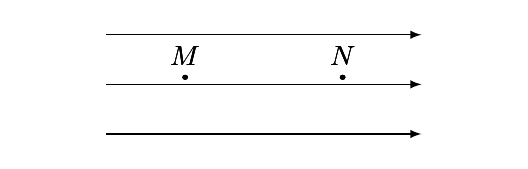
\begin{tikzpicture}[>=latex,yscale=0.9]
  \useasboundingbox(-1,1.2)rectangle(5,2.8);
  \foreach \x in {1.3,2,2.7}
  {
    \draw[->] (0, \x)--(4,\x);
    \node at (1, 2.4){$M$};  \node at (3, 2.4){$N$};
    \fill (1,2.1) circle (1pt); \fill (3,2.1) circle (1pt);
  }
\end{tikzpicture}
\end{document}